\documentclass[./main.tex]{subfiles}
\begin{document}

% Slide # 6
\begin{frame}[t, label=slide06]
        % Title
        \frametitle{\alf{Inferring critical transitions from timeseries}}

        % Body
        \footnotesize

        \begin{equation*}
             f(X_{t};\mu) = -\mu - X_{t}^{2}\quad\Longrightarrow\quad\text{Var}[X_{t}] = \frac{D}{\theta}\to 
                          \begin{cases}
                                0\,, \quad\mu\to\ - \infty\,,\\
                                \infty\,, \quad\mu\to 0\,.
                          \end{cases}
        \end{equation*}

        \begin{figure}[H]
            \centering
            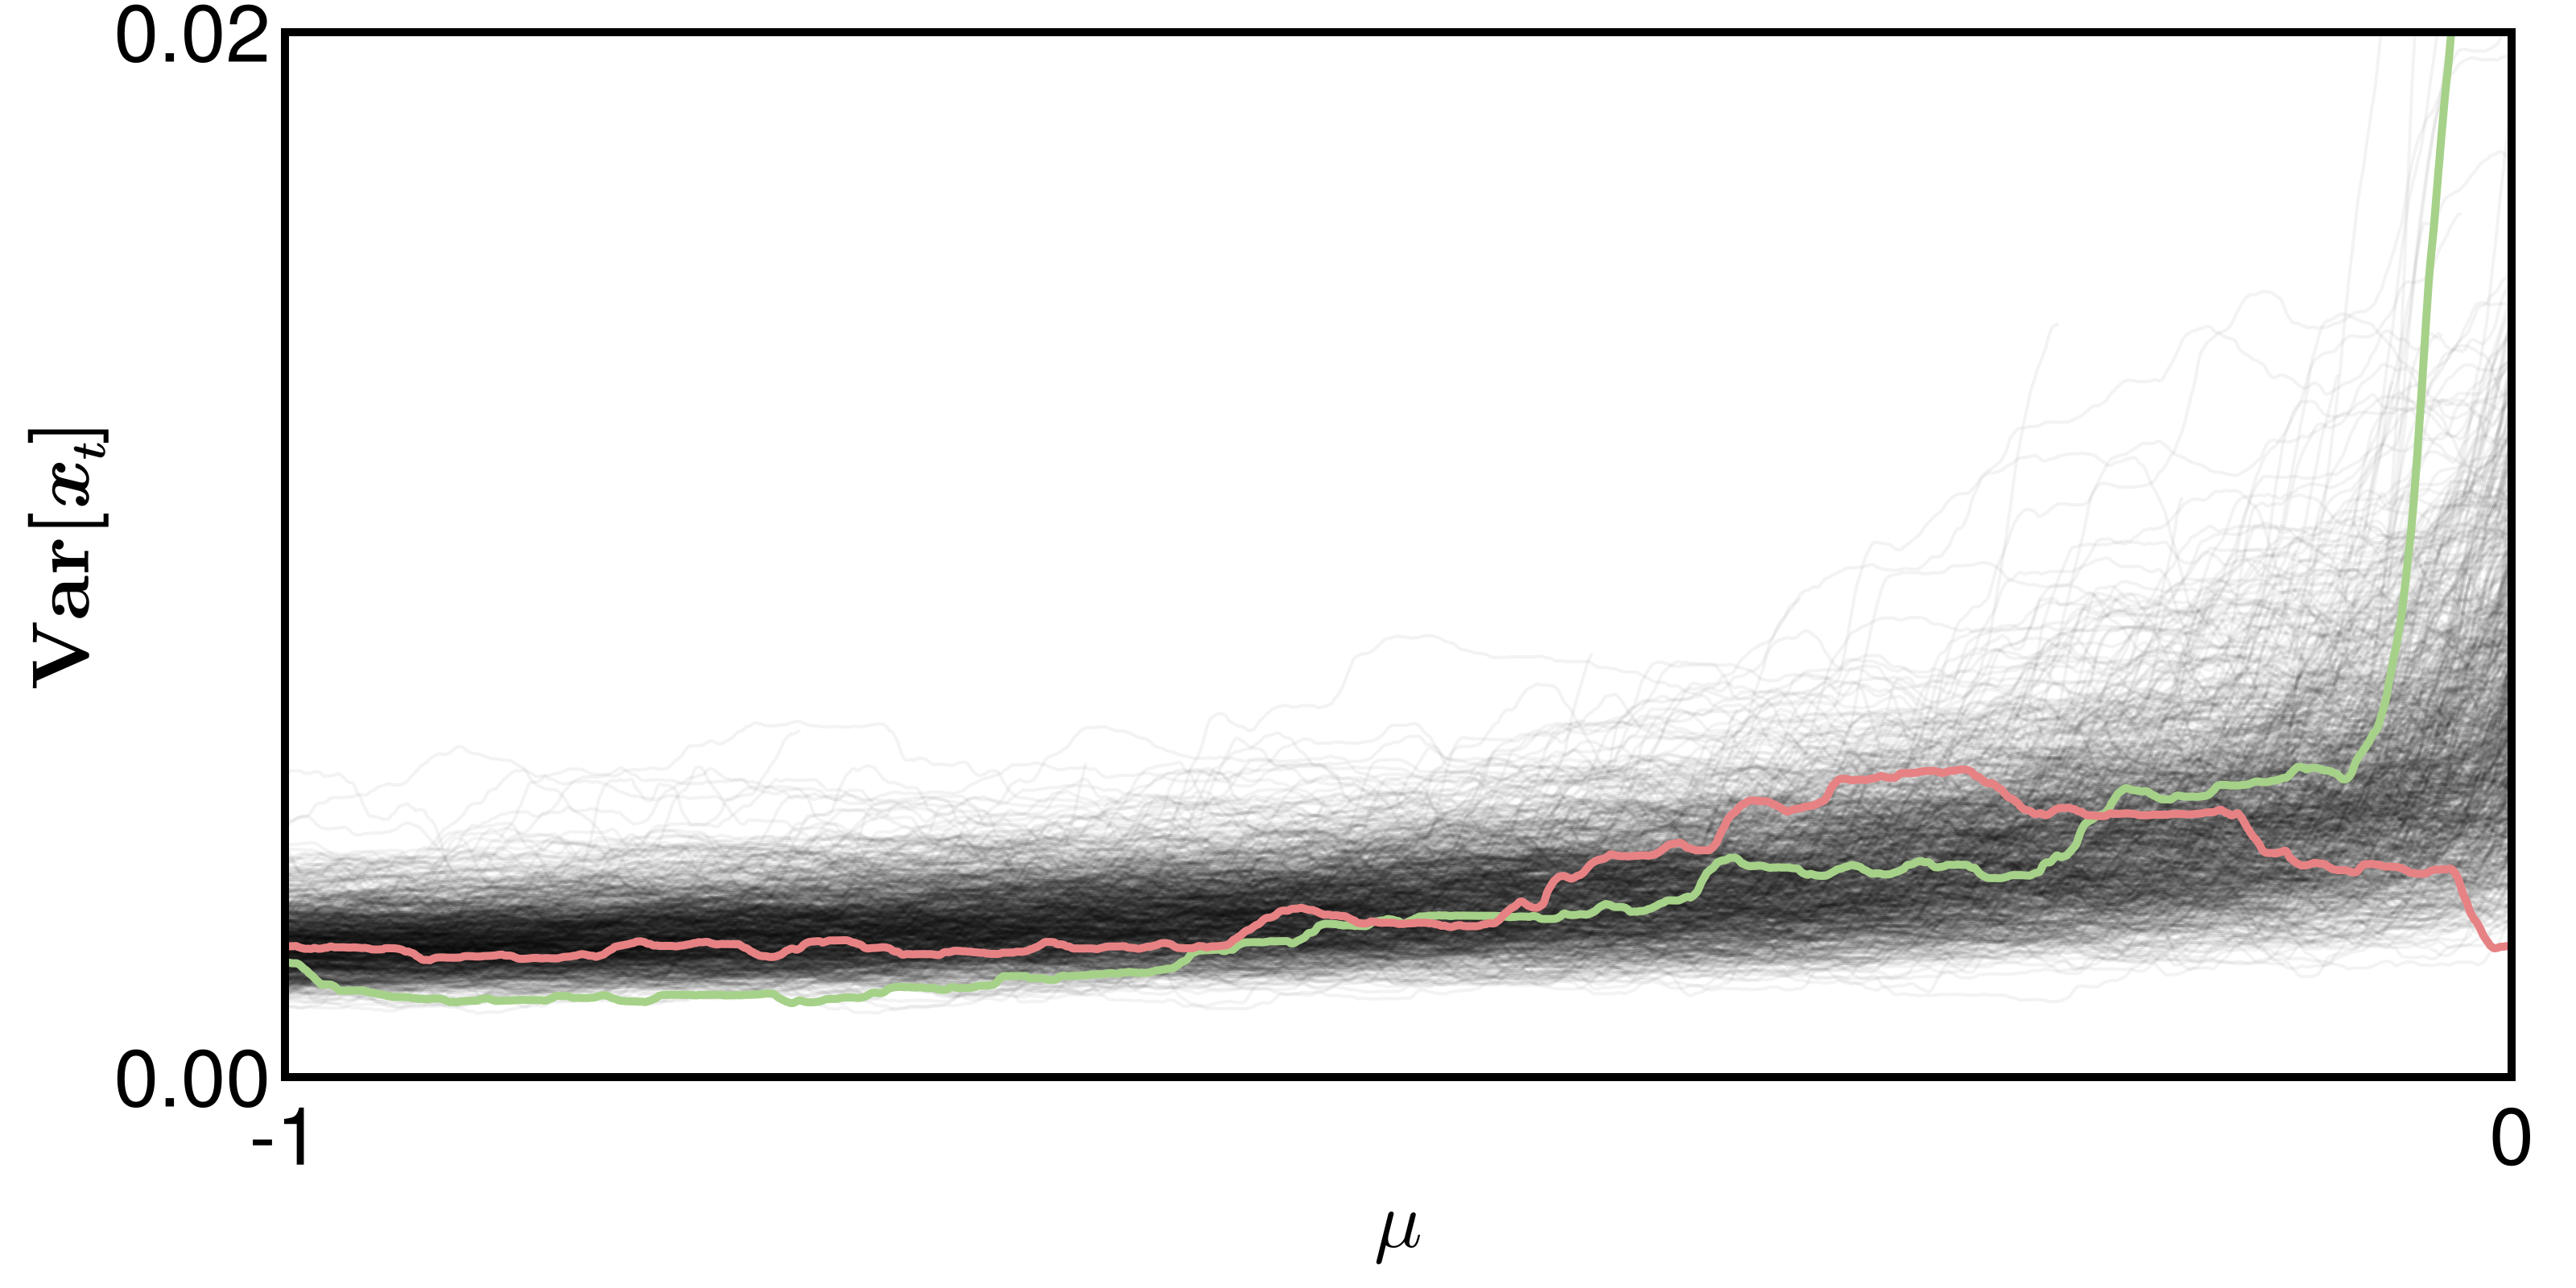
\includegraphics[keepaspectratio, width=\textwidth]{./figures/slide_07.png}%
        \end{figure}
\end{frame}

\end{document}
